\documentclass[10pt,twocolumn]{article}

\usepackage[a4paper,top=17mm,bottom=19mm,left=16mm,right=16mm,columnsep=7mm]{geometry}
\usepackage[T1]{fontenc}
\usepackage{newtxtext,newtxmath}
\usepackage{microtype}
\usepackage{graphicx}
\usepackage{booktabs}
\usepackage{array}
\usepackage{amsmath}
\usepackage{siunitx}
\usepackage{xcolor}
\usepackage{caption}
\usepackage{subcaption}
\usepackage{cuted}
\usepackage{tabularx}
\usepackage{placeins}
\usepackage[numbers,sort&compress]{natbib}
\renewcommand{\bibfont}{\footnotesize}
\setlength{\bibsep}{1.5pt plus 0.5pt}
\usepackage[colorlinks=true,allcolors=blue!55!black]{hyperref}

\definecolor{YouthBlue}{HTML}{1F77B4}
\definecolor{SoftGray}{HTML}{F1F3F5}
\definecolor{TextGray}{HTML}{4D5156}

\captionsetup{font=footnotesize,labelfont=bf,justification=justified,singlelinecheck=false}
\setlength{\parindent}{1em}
\setlength{\parskip}{0pt}
\setlength{\textfloatsep}{8pt plus 2pt minus 2pt}
\setlength{\floatsep}{7pt plus 2pt minus 2pt}
\setlength{\intextsep}{7pt plus 2pt minus 2pt}
\setlength{\stripsep}{6pt plus 1pt minus 1pt}
\sisetup{detect-all,round-mode=places,round-precision=4}
\providecommand{\tightlist}{\setlength{\itemsep}{0pt}\setlength{\parskip}{0pt}}
\makeatletter
\setlength{\@fptop}{0pt}
\makeatother

\begin{document}
\raggedbottom

\twocolumn[
\begin{@twocolumnfalse}
\begin{center}
{\LARGE\bfseries A Donor-Level MSC Youth Score Framework Reveals Trade-offs\par}
\vspace{2pt}
{\Large\bfseries in Small-Cohort Aging-State Modeling\par}
\vspace{8pt}
{\large Zihan Zhou}\par
\vspace{10pt}
\end{center}
\vspace{8pt}
\hrule
\vspace{10pt}
\end{@twocolumnfalse}
]

\section*{Abstract}

Single-cell transcriptomic studies of mesenchymal stromal/stem cell (MSC) aging often contain many cells but few independent donors, creating a tension between apparent predictive performance and donor-level generalizability. We developed a donor-level Youth Score framework that aggregates raw single-cell counts into mouse pseudobulk profiles, estimates sex-compatible age effects with factorial differential-expression models, and uses nested stability selection to construct weighted young-high and old-high gene modules. Fully nested leave-one-mouse-out (LOMO) analysis was used so that filtering, normalization, feature selection, weighting, standardization, and calibration were rebuilt without the held-out mouse.

Controlled ablations showed that age discrimination, within-old age ordering, technical association, and fold-level signature stability reached their strongest values in different model branches. We therefore froze two scientifically distinct models: M1, a 58-gene primary operational reference selected at an inner-fold frequency threshold of \(\pi_g\geq0.75\), and M4, a 29-gene post-ablation high-stringency sensitivity model selected at \(\pi_g\geq0.90\). Both achieved nested LOMO AUC 1.000. Their all-age Spearman correlations were \(-0.806\) and \(-0.844\), respectively, while correlations with raw library size remained substantial (\(-0.692\) and \(-0.727\)). In 999 fully nested, sex-stratified age-label permutations, the prespecified absolute all-age correlations exceeded the randomized-label null for M1 (\(p=0.023\)) and M4 (\(p=0.010\)).

Frozen application to GSE176206 preserved the young-higher-than-aged direction in two control arms and produced negative median SOKM-minus-control contrasts in both age groups. Frozen application to TMS Droplet preserved young-old separation, negative age ordering, and complete signature coverage across assay. M1 and M4 remained highly concordant in GSE176206 and Droplet, and paired Droplet bootstrap intervals did not establish a performance difference between them. These results support a rigorously characterized MSC youth-associated transcriptional-state framework. They also expose a central small-cohort constraint: stronger descriptive trajectory ordering can accompany stronger technical coupling and lower fold-level signature overlap.

\section{Introduction}\label{introduction}

\subsection{Biological and statistical problem}\label{biological-and-statistical-problem}

Quantifying a young-like MSC transcriptional state could support studies of aging, regenerative interventions, and partial reprogramming. The available single-cell datasets create a specific statistical challenge: thousands of cellular measurements may arise from only a small number of biologically independent animals. Treating cells as replicates inflates effective sample size and allows donor-specific, technical, or cohort-specific structure to masquerade as generalizable age biology.

Partial-reprogramming experiments further show why youth-associated expression and cell identity require separate interpretation. \citet{roux2022} reported partial-reprogramming-associated restoration of youthful expression programs together with transient suppression of somatic identity programs in murine systems. This biological separation motivates a Youth-state score whose response is interpreted alongside independent identity and risk axes.

Initial exploratory work showed that three objectives require separate evaluation in these cohorts:

\begin{enumerate}
\def\labelenumi{\arabic{enumi}.}
\tightlist
\item
  \textbf{young-old discrimination}, or separation of broad cohort states;
\item
  \textbf{age ordering}, including ordering among older donors;
\item
  \textbf{robustness}, covering technical association and feature-selection stability.
\end{enumerate}

The final framework addresses these objectives at the donor level and treats technical association as an explicit model diagnostic. Earlier Droplet and FACS models supplied feasibility evidence and exposed donor imbalance, sex-age structure, assay depth, and subtissue contamination as consequential sources of uncertainty. The manuscript analysis begins from the cleaned FACS cohort and uses earlier model behavior only as motivation for prespecified ablations.

\subsection{Contribution}\label{contribution}

We establish a donor-level MSC Youth Score framework with three linked contributions:

\begin{enumerate}
\def\labelenumi{\arabic{enumi}.}
\tightlist
\item
  donor-level pseudobulk scoring with sex-compatible factorial age-effect estimation;
\item
  fully nested stability-controlled feature selection and explicit characterization of the trade-off among age association, technical burden, and signature stability;
\item
  frozen evaluation under regenerative perturbation and cross-assay transfer.
\end{enumerate}

The central methodological finding is a Pareto trade-off under small-cohort constraints. Increasing stability-stringency improved descriptive age ordering in this dataset, while raw-library association strengthened and cross-fold signature Jaccard decreased. The final output is therefore a frozen scoring framework with a primary operational model and a high-stringency sensitivity model, each assigned a distinct evidential role.

\section{Methods}\label{methods}

\subsection{Training cohort and metadata audit}\label{training-cohort-and-metadata-audit}

The final training cohort contained 815 FACS-profiled TMS limb-muscle MSCs from 14 mice after removal of 120 diaphragm cells that were confined to old animals. All retained cells had standardized forelimb/hindlimb subtissue labels. The expression matrix contained 22,966 genes.

\noindent\begin{minipage}{\columnwidth}
\centering
\footnotesize
\captionof{table}{Composition of the cleaned FACS training cohort. The upper panel reports donor counts; the lower panel reports cell counts.}
\label{tab:training-cohort}
\begin{tabular*}{\columnwidth}{@{\extracolsep{\fill}}lrr@{}}
\toprule
Age & Female mice & Male mice \\
\midrule
3 months & 2 & 4 \\
18 months & 2 & 2 \\
24 months & 0 & 4 \\
\bottomrule
\end{tabular*}
\vspace{3pt}

\begin{tabular*}{\columnwidth}{@{\extracolsep{\fill}}lrr@{}}
\toprule
Age & Female cells & Male cells \\
\midrule
3 months & 130 & 134 \\
18 months & 158 & 76 \\
24 months & 0 & 317 \\
\bottomrule
\end{tabular*}
\end{minipage}\par\medskip

The 24-month group contains only male mice. The factorial design supports female and male young-old contrasts, while a female 18-to-24-month trajectory is unidentifiable. Four outer folds were retained with explicit weak-support flags because one factorial cell had only one training mouse. Matrix counts were used as the expression source of truth; two small metadata \texttt{n\_counts} discrepancies in donor \texttt{24\_59\_M} did not alter the pseudobulk matrix or model output.

\subsection{Donor-level pseudobulk}\label{donor-level-pseudobulk}

Raw single-cell counts were summed within each mouse:

\[
C_{gm}=\sum_{c\in m} C_{gc},
\]

where \(C_{gc}\) is the raw count for gene \(g\) in cell \(c\), and \(C_{gm}\) is the mouse-level pseudobulk count. Cells are measurement units; mice are inference and validation units.

This sum-based pseudobulk preserves the count scale required by edgeR TMM and limma-voom. It also prevents donor cell abundance from being converted into artificial biological replication.

\subsection{Training-partition filtering, TMM, and voom}\label{training-partition-filtering-tmm-and-voom}

Within every training partition, gene \(g\) was retained when

\[
\mathrm{CPM}_{gm}>1
\]

in at least two training mice. Outer LOMO folds retained 12,535 to 12,777 genes, with a median of 12,708. TMM factors and the voom mean-variance relationship were estimated from the training mice only. TMM and voom were used for differential-expression estimation; deployment scoring used the frozen raw all-gene transform described below.

PCA was used as exploratory quality control for age, sex, library size, detected genes, and cell count. It did not determine signature membership.

\subsection{Sex-compatible age-effect estimation}\label{sex-compatible-age-effect-estimation}

An age-only model supplied a direction-consistency check:

\[
E_g\sim \mathrm{AgeGroup}.
\]

The main differential-expression model was a factorial cell-means design:

\[
E_g\sim 0+\mathrm{Sex}:\mathrm{AgeGroup}.
\]

For each gene, female, male, common, and interaction effects were defined as

\[
\beta_{g,F}=\mu_{g,F,O}-\mu_{g,F,Y},
\]

\[
\beta_{g,M}=\mu_{g,M,O}-\mu_{g,M,Y},
\]

\[
\beta_{g,C}=\frac{\beta_{g,F}+\beta_{g,M}}{2},
\]

\[
\beta_{g,I}=\beta_{g,M}-\beta_{g,F}.
\]

Genes entered the reliability pool when female and male effects shared a nonzero direction, the age-only and common factorial effects shared a nonzero direction, common statistics were finite, and the gene was absent from the frozen sex-linked exclusion list. This construction emphasizes age effects that remain directionally compatible across sex despite the unbalanced age-by-sex cohort.

\subsection{Interaction-aware ranking}\label{interaction-aware-ranking}

Sex heterogeneity was summarized by

\[
R_g=\frac{|\beta_{g,I}|}{|\beta_{g,F}|+|\beta_{g,M}|+\epsilon},
\]

with interaction penalty

\[
P_g=\frac{1}{1+R_g}.
\]

Eligible genes were ranked by

\[
w_g=|\beta_{g,C}|\,|t_{g,C}|\,P_g,
\]

where \(t_{g,C}\) is the moderated common-effect statistic. Genes with \(\beta_{g,C}<0\) formed the young-high module; genes with \(\beta_{g,C}>0\) formed the old-high module.

\subsection{Nested stability selection}\label{nested-stability-selection}

Inside each outer-training partition, provisional signatures were reconstructed in inner LOMO folds, with at most 50 genes per direction in each provisional signature. This cap stabilized inner-fold ranking under the very small donor count and was fixed before external application; it was not tuned against external performance. Gene-level selection frequency was

\[
\pi_g=
\frac{\text{eligible inner folds selecting }g}
{\text{number of eligible inner folds}}.
\]

M1 retained genes with \(\pi_g\geq0.75\). M4 retained genes with \(\pi_g\geq0.90\). The stable pool was reranked on the complete outer-training partition, capped at 100 genes per module, and never backfilled with genes below the frozen frequency threshold. Rank-deficient inner splits were recorded and skipped without changing the factorial model.

\subsection{Frozen scoring function}\label{frozen-scoring-function}

M1 and M4 use the raw all-gene library denominator:

\[
X_{gm}=
\log_2\left(
10^6\frac{C_{gm}}{\sum_{h\in G_{all}}C_{hm}}+1
\right).
\]

Gene values were standardized using training-only parameters:

\[
Z_{gm}=\frac{X_{gm}-\mu_g^{train}}{s_g^{train}}.
\]

For module \(A\), the weighted module score was

\[
S_A(m)=
\frac{\sum_{g\in A}w_gZ_{gm}}
{\sum_{g\in A}w_g}.
\]

The raw Youth Score was

\[
Y_m^{raw}=S_{young}(m)-S_{old}(m).
\]

Let \(M_Y\) and \(M_O\) be the median raw scores among young and old training mice. The calibrated score was

\[
Y_m=
\frac{Y_m^{raw}-M_O}{M_Y-M_O}.
\]

Training medians are fixed to 1 for young and 0 for old by construction. Model evaluation therefore uses held-out LOMO scores or frozen external applications.

\subsection{Fully nested donor-level validation}\label{fully-nested-donor-level-validation}

For every held-out mouse, the complete training-side pipeline was rebuilt:

\begin{enumerate}
\def\labelenumi{\arabic{enumi}.}
\tightlist
\item
  gene filtering;
\item
  TMM and voom estimation;
\item
  age-only and factorial differential expression;
\item
  reliability screening and interaction-aware ranking;
\item
  inner LOMO stability selection;
\item
  module selection and weight estimation;
\item
  training-only standardization and calibration;
\item
  frozen-transform scoring of the untouched held-out mouse.
\end{enumerate}

This design prevents feature-selection, normalization, and calibration leakage. Performance was summarized by young-old AUC, all-age Spearman correlation, old-only Spearman correlation, young-old median difference, associations with technical variables, signature size, and fold Jaccard.

\subsection{Controlled ablation design and operating points}\label{controlled-ablation-design-and-operating-points}

The exact historical factorial stability-selected implementation was retained as M0, a sanity anchor for testing whether later changes altered the established donor ordering. Three independent design questions were then evaluated:

\noindent\begin{minipage}{\columnwidth}
\centering
\footnotesize
\captionof{table}{Controlled ablation design and prespecified model roles.}
\label{tab:ablation-design}
\begin{tabularx}{\columnwidth}{@{}l X@{}}
\toprule
Analysis & Role and design question \\
\midrule
M1 & \textit{Role:} Primary operating point \newline \textit{Design question:} Does correcting the deployment denominator preserve the historical solution? \\
M2 & \textit{Role:} Technical-adjustment ablation \newline \textit{Design question:} Does adding library size and cell count during DE reduce final score-level technical coupling? \\
M3 & \textit{Role:} Stability-threshold sweep \newline \textit{Design question:} How does \(\pi_g=0.50\), 0.75, or 0.90 move the score across age ordering, technical association, and fold stability? \\
M4 & \textit{Role:} High-stringency operating point \newline \textit{Design question:} What behavior is retained when the corrected denominator is combined with \(\pi_g\geq0.90\)? \\
\bottomrule
\end{tabularx}
\end{minipage}\par\medskip

M1, M2, and M3 branch independently from M0. M2 retains the M0 normalization contract, so its effect isolates the DE adjustment. M4 was frozen after review of the independent ablations and retains a post-ablation exploratory role. Complete branch definitions and results are reported in Appendices A-C.

\subsection{Frozen permutation test}\label{frozen-permutation-test}

The primary permutation statistic was

\[
T_{\rho}=|\rho(Y,\mathrm{Age})|.
\]

Complete 3-, 18-, and 24-month labels were reassigned within sex strata. Every assignment reran the fully nested pipeline, including feature selection and calibration. The empirical two-sided p-value was

\[
p=\frac{1+\sum_{b=1}^{999}I(T_b\geq T_{obs})}{1000}.
\]

All 999 assignments were unique and valid for both models. Young-old AUC distance from 0.5 was prespecified as supporting evidence; young-old median difference was recorded as a non-primary statistic.

\subsection{Frozen external application}\label{frozen-external-application}

External datasets were never used to change genes, weights, standardization, calibration, thresholds, or score orientation.

For GSE176206, the MSC SOKM object contained 20,661 source cells, of which 18,686 met the frozen analysis criteria and formed 18 age-treatment-animal units. Raw counts from \texttt{layers{[}\textquotesingle{}counts\textquotesingle{}{]}} were aggregated by age, exact treatment arm, and nested animal identifier. Numeric animal labels were treated as nested within each exact arm, so treatment comparisons were unpaired. The source study profiled young and aged murine MSCs after transient SOKM induction and chase; the present analysis used this dataset to assess baseline age direction and perturbation-related biological consistency \citep{roux2022,geo176206}.

For TMS Droplet, the frozen models were applied to 12 mouse-level pseudobulk profiles: two at 3 months, four at 18 months, two at 21 months, and four at 24 months. The 20,138-gene all-gene column sum supplied the parser denominator. This analysis assessed within-TMS cross-assay transportability. Paired donor bootstrap compared M4-minus-M1 differences without model reselection.

\section{Results}\label{results}

\subsection{Small-cohort evaluation exposes multiple optimization objectives}\label{small-cohort-evaluation-exposes-multiple-optimization-objectives}

Controlled ablations were designed to identify representative operating points across competing objectives. The diagnostic branches separated broad age discrimination from within-old ordering, technical association, and signature stability. Every model retained 14 valid held-out scores and zero empty outer signatures.

M0 served as a provenance anchor, establishing the reproducible v2.1 solution as the fixed baseline for every subsequent v3.1 modification.

\noindent\begin{minipage}{\columnwidth}
\centering
\footnotesize
\captionof{table}{Summary of the controlled ablation branches.}
\label{tab:ablation-summary}
\begin{tabularx}{\columnwidth}{@{}l X@{}}
\toprule
Analysis & Main change and key observation \\
\midrule
M1 & \textit{Main change:} Corrected raw all-gene denominator at \(\pi_g\geq0.75\) \newline \textit{Key observation:} Preserved the historical donor ranking and supplied the primary operational reference \\
M2 & \textit{Main change:} Added library size and cell count during DE \newline \textit{Key observation:} Produced limited raw-library improvement while weakening age ordering and increasing cell-count coupling \\
M3 & \textit{Main change:} Swept \(\pi_g\) from 0.50 to 0.90 \newline \textit{Key observation:} Showed that higher stringency strengthened descriptive age ordering while increasing raw-library coupling and lowering fold Jaccard \\
M4 & \textit{Main change:} Combined the corrected denominator with \(\pi_g\geq0.90\) \newline \textit{Key observation:} Defined a representative high-stringency operating point for sensitivity analysis \\
\bottomrule
\end{tabularx}
\end{minipage}\par\medskip

M1 preserved the M0 donor ranks after correcting the deployment denominator. This correction separated scoring normalization from training-fold gene filtering without changing the learned donor ordering. M2 supplied the central technical-adjustment control: raw-library correlation improved only modestly, while old-only ordering changed from \(-0.109\) to \(+0.436\) and cell-count association strengthened. The M3 threshold sweep then identified stability stringency as the design factor that moved the score toward stronger descriptive age ordering, accompanied by stronger raw-library coupling and lower fold stability.

\begin{figure*}[t]
\begin{minipage}[t]{0.56\textwidth}
\centering
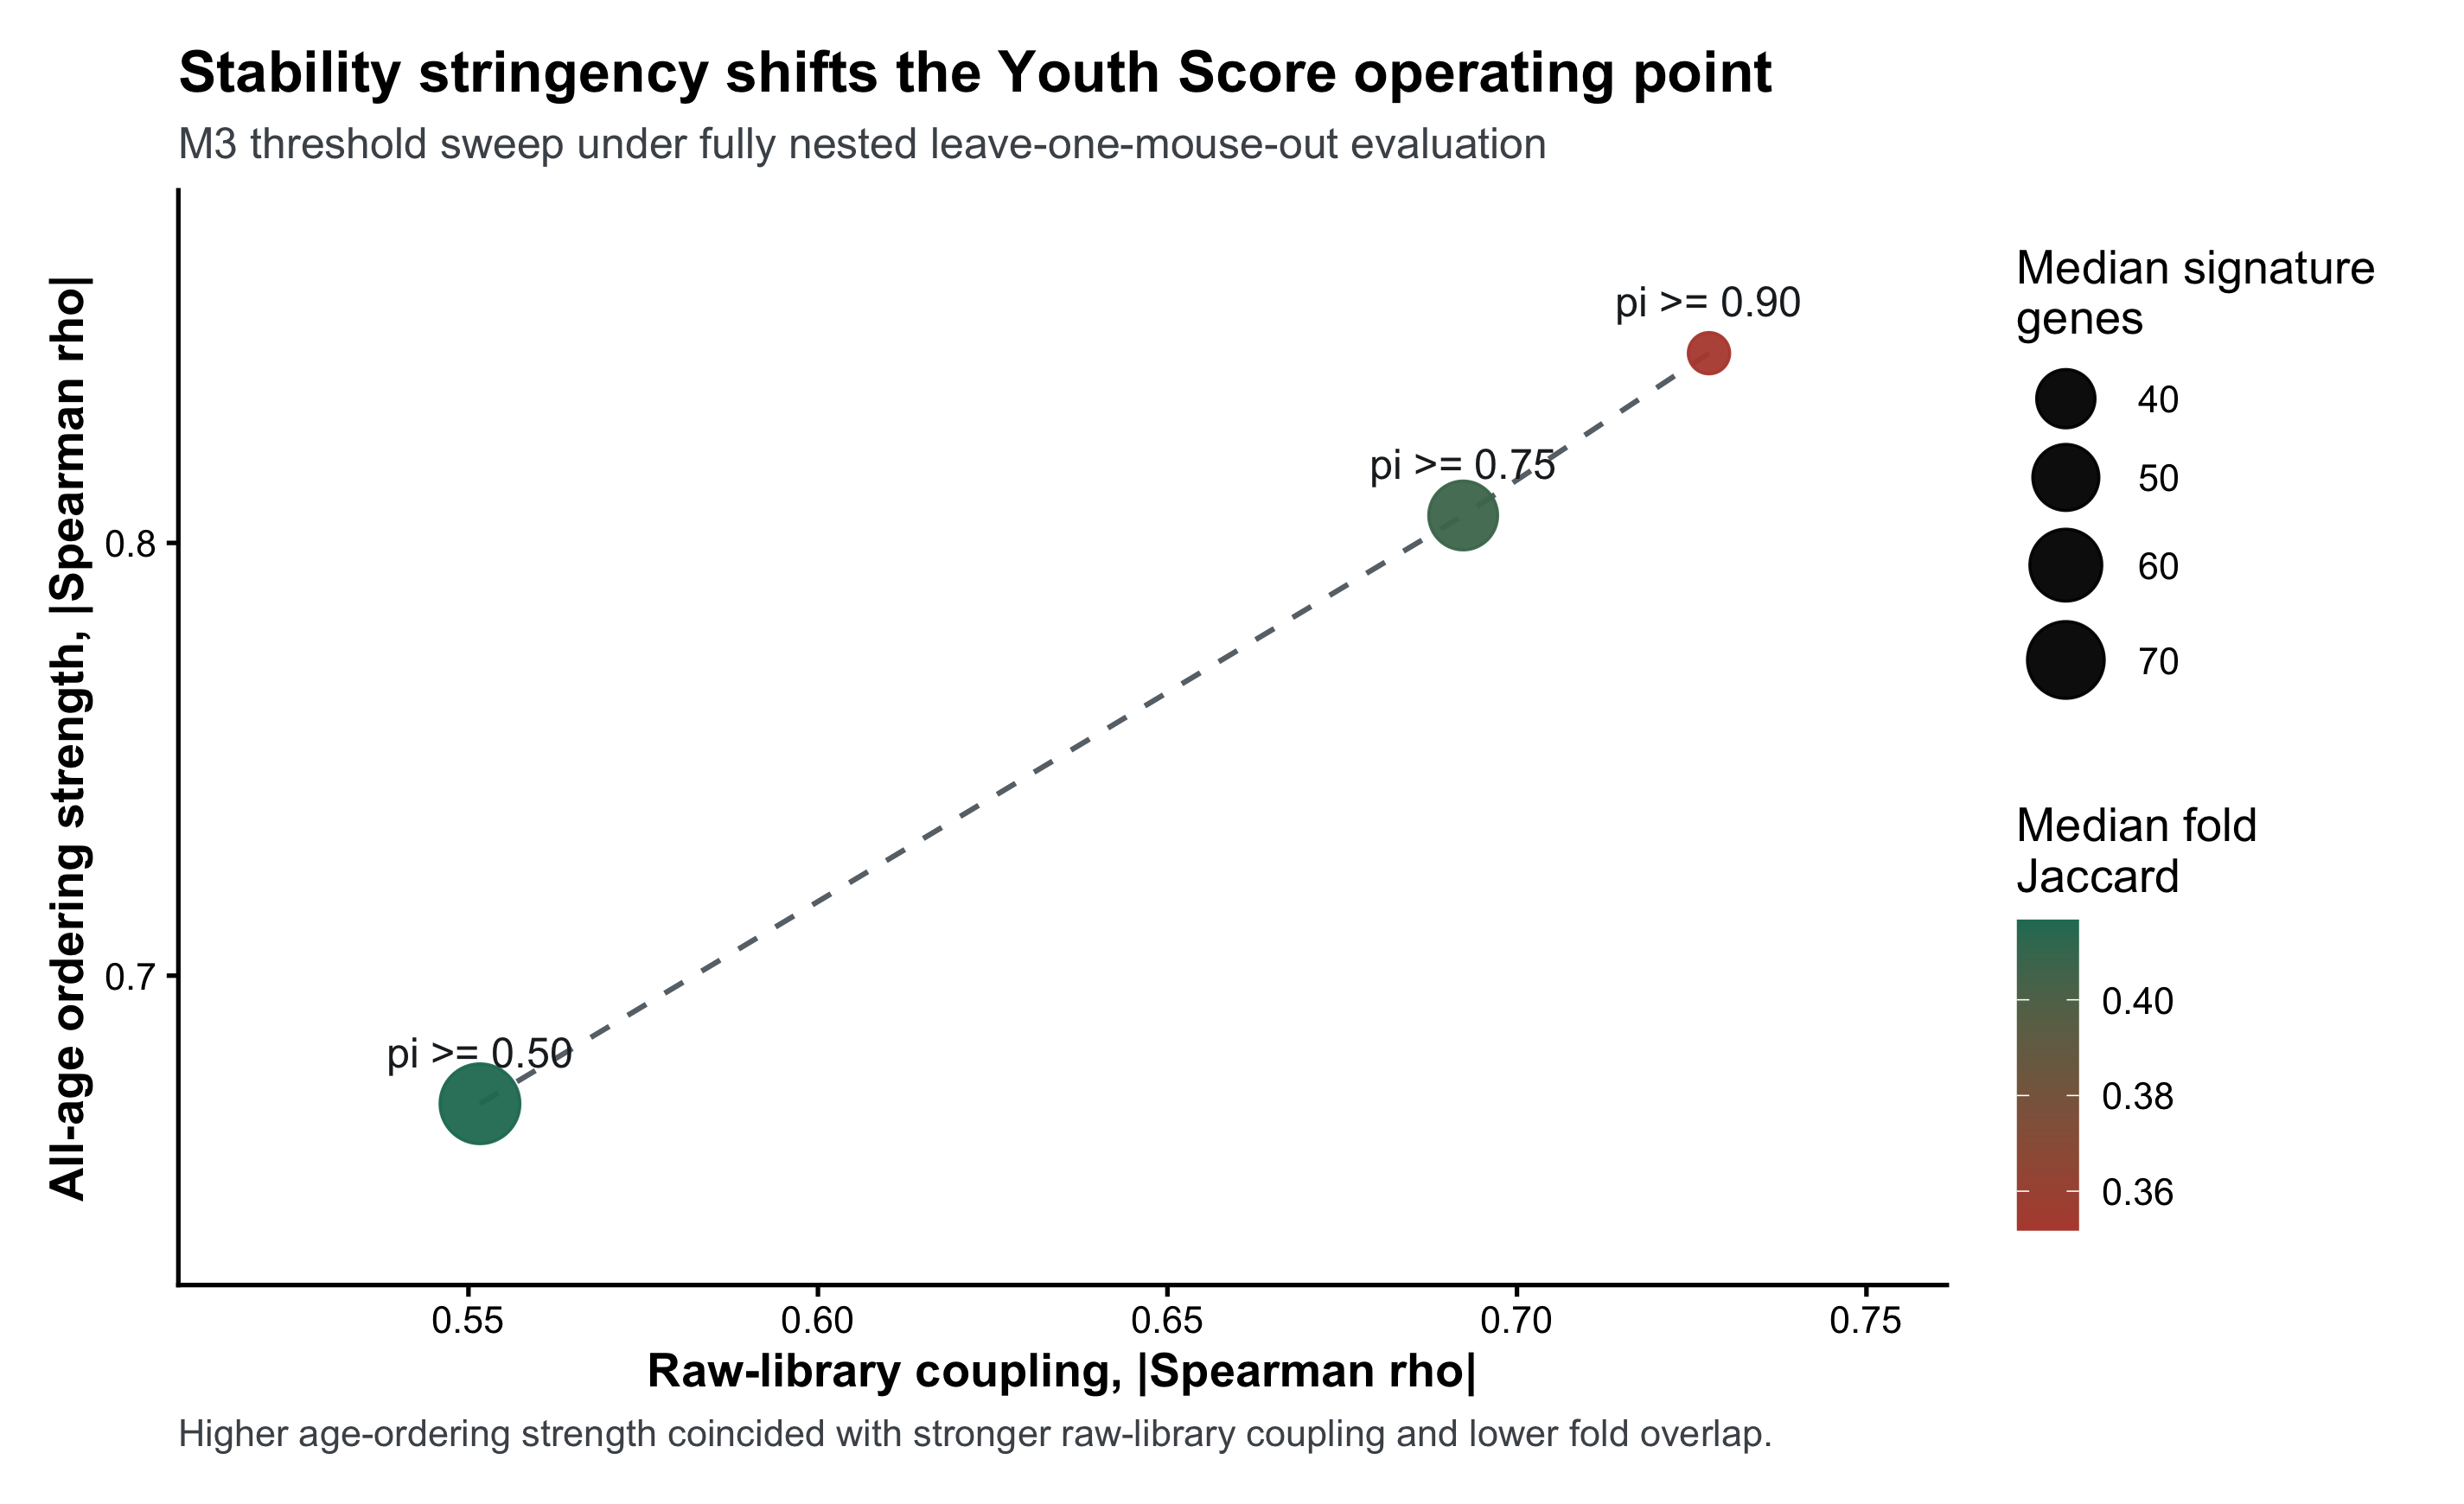
\includegraphics[width=\linewidth]{figures/manuscript_stability_tradeoff.png}
\captionof{figure}{Stability-threshold trade-off under nested LOMO.}
\label{fig:stability-tradeoff}
\end{minipage}\hfill
\begin{minipage}[t]{0.40\textwidth}
\centering
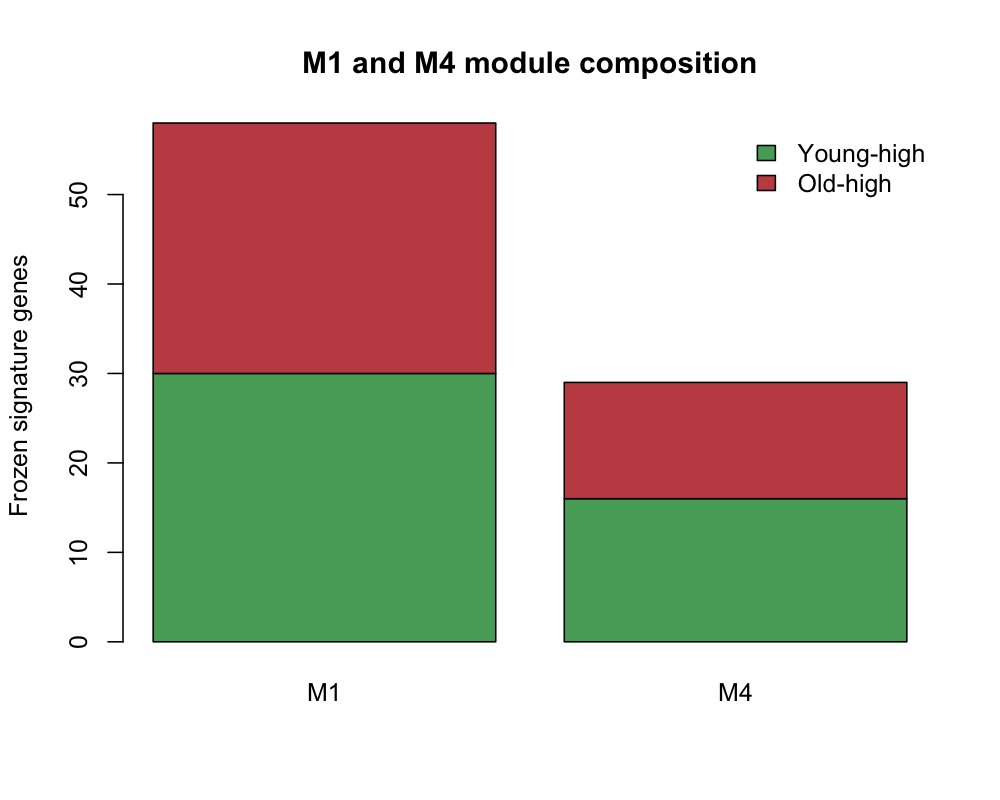
\includegraphics[width=\linewidth]{figures/frozen_signature_module_composition.png}
\captionof{figure}{Frozen signature composition.}
\label{fig:signature-composition}
\end{minipage}
\end{figure*}

Together, these ablations explain the selection of M1 and M4 as representative operating points. Complete M0-M4 metrics, denominator-equivalence results, and threshold-sweep values are reported in Appendices A-C.

\subsection{Two frozen models define representative operating points}\label{two-frozen-models-define-representative-operating-points}

Full-data freezing selected 58 genes for M1, comprising 30 young-high and 28 old-high genes, and 29 genes for M4, comprising 16 young-high and 13 old-high genes. Calibration denominators were 2.65029 and 2.70224.

\noindent\begin{minipage}{\columnwidth}
\centering
\footnotesize
\captionof{table}{Fully nested LOMO performance of the frozen operating points. The upper panel gives model roles; the lower panel gives nested performance.}
\label{tab:frozen-candidates}
\begin{tabularx}{\columnwidth}{@{}l X@{}}
\toprule
Model & Frozen role \\
\midrule
M1 & Primary operational reference \\
M4 & High-stringency sensitivity model \\
\bottomrule
\end{tabularx}
\vspace{3pt}

\scriptsize
\begin{tabular*}{\columnwidth}{@{\extracolsep{\fill}}lrrrrr@{}}
\toprule
Model & Stability threshold & Genes & Nested AUC & All-age \(\rho\) & Old-only \(\rho\) \\
\midrule
M1 & 0.75 & 58 & 1.000 & -0.806 & -0.109 \\
M4 & 0.90 & 29 & 1.000 & -0.844 & -0.327 \\
\bottomrule
\end{tabular*}
\end{minipage}\par\medskip

M1 preserves the corrected deployment transform and the broader stable pool. M4 emphasizes genes selected in at least 90\% of eligible inner folds and provides a trajectory-sensitive operating point. M4\textquotesingle s development followed review of the ablations, so its favorable internal point estimates remain exploratory evidence.

M4 was retained to quantify how conclusions change under a stricter stability constraint. This sensitivity role tests robustness to feature-stringency while preserving M1 as the primary operational reference.

\begin{figure*}[t]
\centering
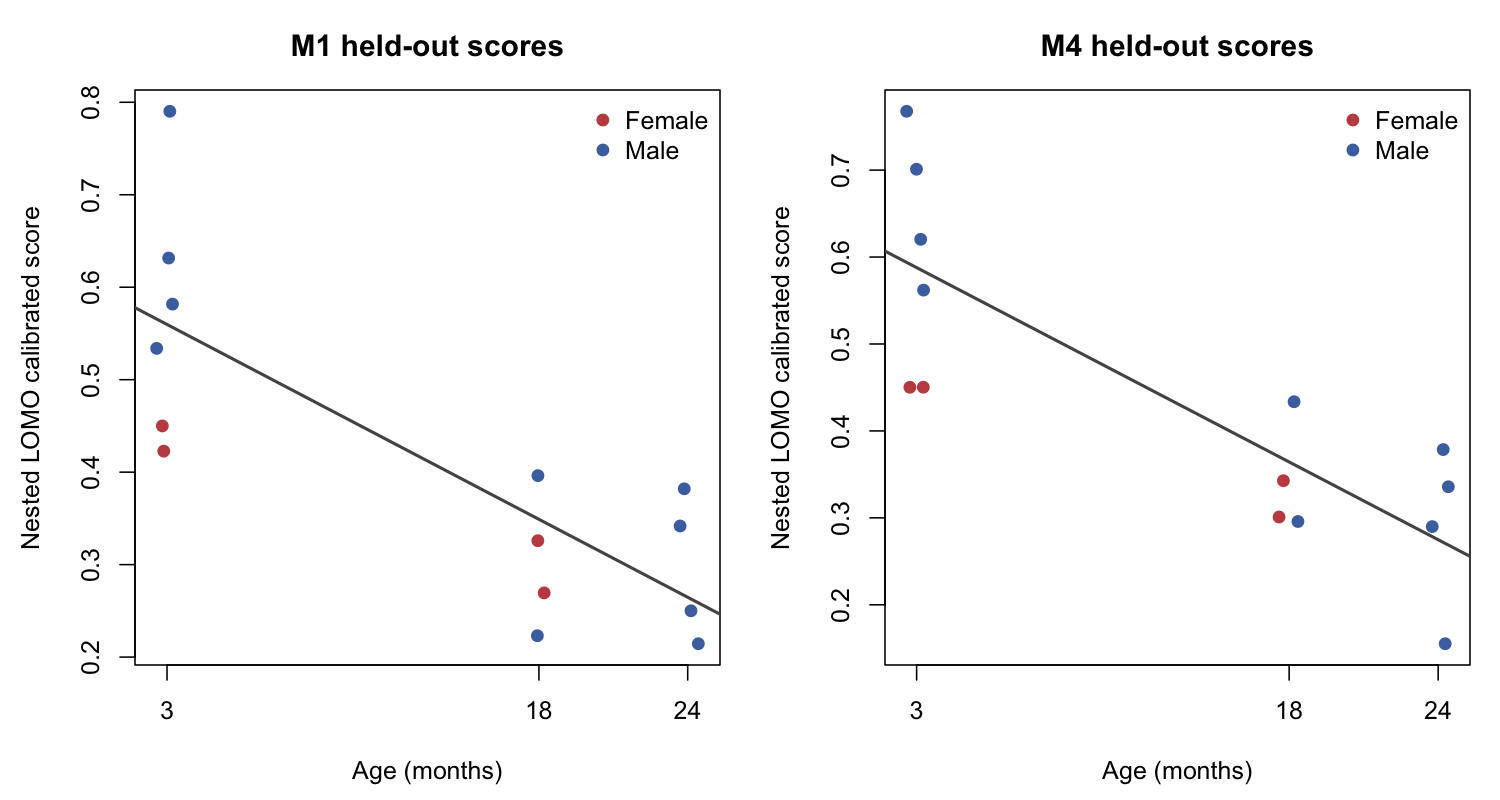
\includegraphics[width=0.72\textwidth]{figures/training_nested_lomo_scores_by_age.png}
\caption{Nested LOMO scores for the frozen candidates.}
\label{fig:nested-lomo}
\end{figure*}

\subsection{Frozen nested pipelines exceed randomized-age nulls}\label{frozen-nested-pipelines-exceed-randomized-age-nulls}

The 999 sex-stratified permutations reconstructed every model component within each outer fold. All assignments produced 14 valid scores per model, preserved sex-age counts, and had no zero-signature or rank-deficient outer folds.

\noindent\begin{minipage}{\columnwidth}
\centering
\footnotesize
\captionof{table}{Observed nested statistics and sex-stratified permutation nulls. The upper panel reports observed statistics; the lower panel reports their permutation-null summaries.}
\label{tab:permutation}
\begin{tabular*}{\columnwidth}{@{\extracolsep{\fill}}llr@{}}
\toprule
Model & Statistic & Observed \\
\midrule
M1 & \(\rho_{age}\) & 0.806 \\
M1 & \(\mathrm{AUC}-0.5\) & 0.500 \\
M4 & \(\rho_{age}\) & 0.844 \\
M4 & \(\mathrm{AUC}-0.5\) & 0.500 \\
\bottomrule
\end{tabular*}
\vspace{3pt}

\scriptsize
\begin{tabular*}{\columnwidth}{@{\extracolsep{\fill}}llrrrr@{}}
\toprule
Model & Statistic & Null mean & Null SD & \(Z_{null}\) & Empirical \(p\) \\
\midrule
M1 & \(\rho_{age}\) & 0.358 & 0.229 & 1.953 & 0.023 \\
M1 & \(\mathrm{AUC}-0.5\) & 0.218 & 0.138 & 2.036 & 0.039 \\
M4 & \(\rho_{age}\) & 0.355 & 0.225 & 2.177 & 0.010 \\
M4 & \(\mathrm{AUC}-0.5\) & 0.215 & 0.139 & 2.047 & 0.036 \\
\bottomrule
\end{tabular*}
\end{minipage}\par\medskip

The prespecified result supports age-label association beyond the practical randomized-label null for both frozen pipelines. The test addresses label association under the cohort structure; technical independence and continuous-clock validity require separate evidence.

\begin{figure*}[t]
\centering
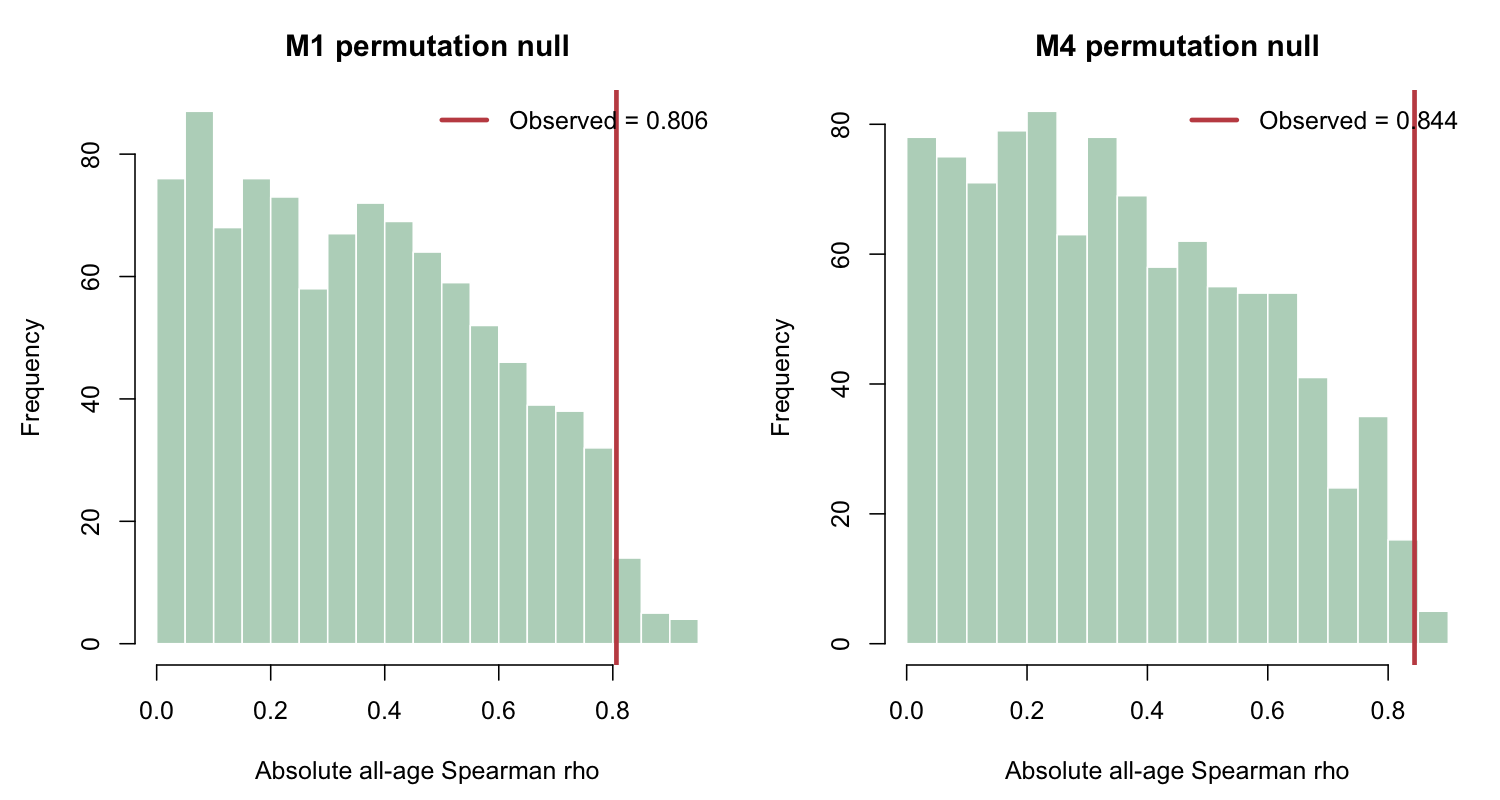
\includegraphics[width=0.72\textwidth]{figures/formal_permutation_abs_all_age_rho_null.png}
\caption{Formal permutation null for absolute all-age correlation.}
\label{fig:permutation-null}
\end{figure*}

\subsection{Frozen evaluation supports biological direction and assay transportability}\label{frozen-evaluation-supports-biological-direction-and-assay-transportability}

\subsubsection{GSE176206 biological application}\label{gse176206-biological-application}

Both models passed total and module-level coverage gates. Minimum module gene and weighted coverage were 0.867 and 0.870 for M1, and 0.938 and 0.922 for M4. In both control arms, median Youth Scores were higher in young than aged animals.

\noindent\begin{minipage}{\columnwidth}
\centering
\footnotesize
\captionof{table}{Baseline age-direction results in the GSE176206 control arms. The upper panel gives age-group medians; the lower panel gives separation metrics.}
\label{tab:gse-baseline}
\begin{tabular*}{\columnwidth}{@{\extracolsep{\fill}}llrr@{}}
\toprule
Model & Control arm & Young median & Aged median \\
\midrule
M1 & \texttt{Tg+/Dox-} & 0.4864 & 0.4298 \\
M1 & \texttt{Tg-/Dox+} & 0.5003 & 0.4550 \\
M4 & \texttt{Tg+/Dox-} & 0.4137 & 0.3635 \\
M4 & \texttt{Tg-/Dox+} & 0.4481 & 0.3856 \\
\bottomrule
\end{tabular*}
\vspace{3pt}

\begin{tabular*}{\columnwidth}{@{\extracolsep{\fill}}llrr@{}}
\toprule
Model & Control arm & Young-minus-aged median & AUC \\
\midrule
M1 & \texttt{Tg+/Dox-} & 0.0566 & 1.000 \\
M1 & \texttt{Tg-/Dox+} & 0.0453 & 0.778 \\
M4 & \texttt{Tg+/Dox-} & 0.0503 & 1.000 \\
M4 & \texttt{Tg-/Dox+} & 0.0626 & 0.778 \\
\bottomrule
\end{tabular*}
\end{minipage}\par\medskip

The prespecified median SOKM-minus-control contrast was negative for both models, both ages, and both control arms.

\noindent\begin{minipage}{\columnwidth}
\centering
\footnotesize
\captionof{table}{Median SOKM-minus-control contrasts in GSE176206.}
\label{tab:gse-sokm-contrast}
\begin{tabular*}{\columnwidth}{@{\extracolsep{\fill}}llrr@{}}
\toprule
Model & Age & Versus \texttt{Tg+/Dox-} & Versus \texttt{Tg-/Dox+} \\
\midrule
M1 & Young & -0.0648 & -0.0787 \\
M1 & Aged & -0.0148 & -0.0400 \\
M4 & Young & -0.0806 & -0.1150 \\
M4 & Aged & -0.0455 & -0.0676 \\
\bottomrule
\end{tabular*}
\end{minipage}\par\medskip

The M1 aged SOKM-versus-\texttt{Tg+/Dox-} mean difference was slightly positive at 0.0042 while the prespecified median difference was -0.0148. The perturbation result is therefore directional median evidence across small unpaired arms, with heterogeneous support across summary statistics.

M1 and M4 had overall Spearman agreement 0.930 and age-treatment-residualized agreement 0.907 across the 18 nested-animal treatment units. State-restricted contrasts were heterogeneous, and pure reprogramming states absent from controls represented composition changes. These observations localize the strongest evidence to an aggregate perturbation-sensitive youth-associated state axis. Formal separation of Youth, MSC identity, and treatment risk awaits independently frozen Identity and Risk scorers.

\begin{figure*}[t]
\begin{minipage}[t]{0.56\textwidth}
\centering
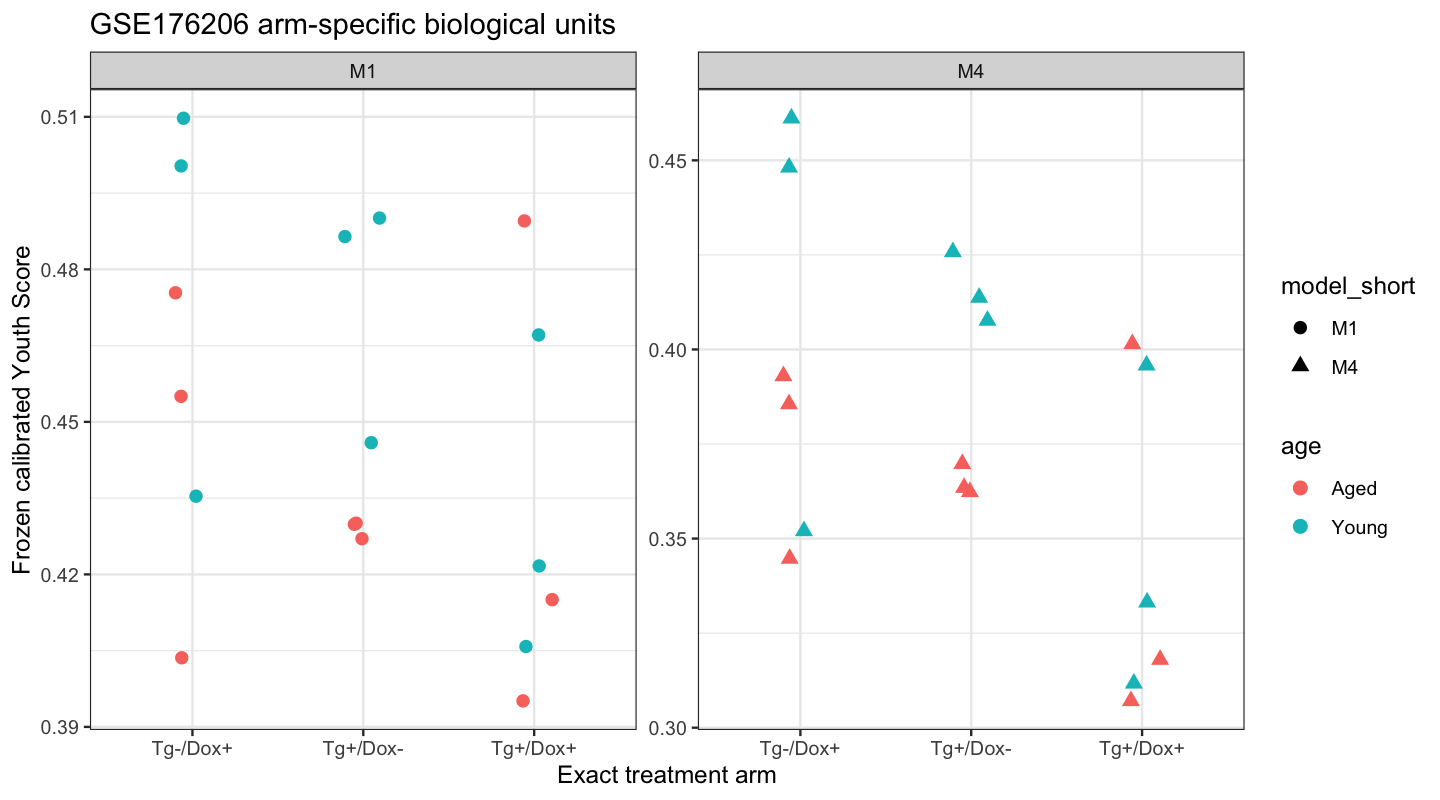
\includegraphics[width=\linewidth]{figures/gse176206_scores_by_exact_treatment.png}
\captionof{figure}{GSE176206 scores by exact treatment.}
\label{fig:gse176206}
\end{minipage}\hfill
\begin{minipage}[t]{0.40\textwidth}
\centering
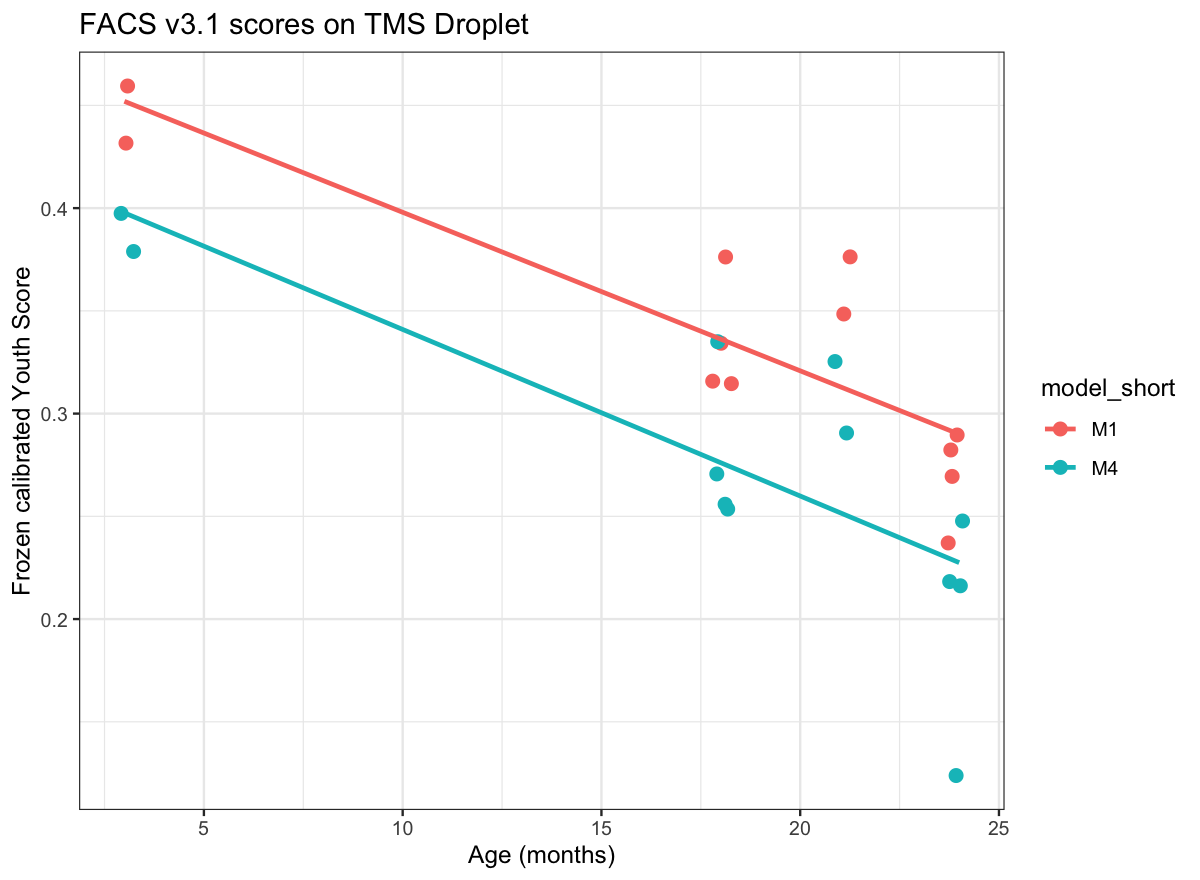
\includegraphics[width=\linewidth]{figures/droplet_scores_by_age.png}
\captionof{figure}{Droplet scores by age.}
\label{fig:droplet}
\end{minipage}
\end{figure*}

\subsubsection{TMS Droplet cross-assay transportability}\label{tms-droplet-cross-assay-transportability}

All M1 and M4 signature genes were present in the Droplet pseudobulk matrix. Both frozen models achieved AUC 1.000, young medians above old medians, and negative all-age and old-only correlations.

\noindent\begin{minipage}{\columnwidth}
\centering
\footnotesize
\captionof{table}{Frozen M1 and M4 transportability metrics in TMS Droplet. The upper panel reports age-related behavior; the lower panel reports technical-variable associations.}
\label{tab:droplet-transport}
\scriptsize
\begin{tabular*}{\columnwidth}{@{\extracolsep{\fill}}lrrrrr@{}}
\toprule
Model & Young median & Old median & AUC & All-age \(\rho\) & Old-only \(\rho\) \\
\midrule
M1 & 0.4455 & 0.3152 & 1.000 & -0.808 & -0.662 \\
M4 & 0.3882 & 0.2547 & 1.000 & -0.830 & -0.701 \\
\bottomrule
\end{tabular*}
\vspace{3pt}

\footnotesize
\begin{tabular*}{\columnwidth}{@{\extracolsep{\fill}}lrrr@{}}
\toprule
Model & All-gene library \(\rho\) & Cell-count \(\rho\) & Detected-gene \(\rho\) \\
\midrule
M1 & -0.028 & -0.098 & 0.336 \\
M4 & -0.035 & -0.105 & 0.308 \\
\bottomrule
\end{tabular*}
\end{minipage}\par\medskip

M1 and M4 donor scores had overall Spearman agreement 0.965, old-only agreement 0.939, and exact-age-residualized agreement 0.846. M4 had slightly more negative age-correlation point estimates, while every prespecified paired-bootstrap interval for M4-minus-M1 included zero. The Droplet analysis therefore supports shared cross-assay direction and leaves the frozen model roles unchanged.

\subsection{Frozen parser reproduces the training implementation}\label{frozen-parser-reproduces-the-training-implementation}

The exported parsers reproduced independently computed training scores with maximum calibrated differences of \(2.00\times10^{-15}\) for M1 and \(1.18\times10^{-15}\) for M4. Adding a new sample left existing sample scores unchanged, full-coverage inputs passed, and a deliberately feature-limited input triggered the frozen coverage error.

These controls establish numerical reproducibility and deployable normalization. They complement the inferential analyses without using apparent full-data scores as performance evidence.

\FloatBarrier
\section{Discussion}\label{discussion}

\subsection{A youth-associated state score under small-cohort constraints}\label{a-youth-associated-state-score-under-small-cohort-constraints}

The framework derives a reproducible donor-level youth-associated transcriptional axis within the evaluated MSC cohorts. Its key advance is the integration of sex-compatible effect estimation, inner-fold feature stability, fully nested donor validation, technical diagnostics, and frozen external application. This design addresses the gap between large cell counts and small independent-donor counts that characterizes many single-cell aging datasets.

The formal permutation results show that the frozen pipelines contain stronger age-label association than expected under sex-stratified randomized labels. GSE176206 and Droplet extend this evidence by showing directionally consistent behavior under a regenerative perturbation context and an assay shift. Together, these layers support a characterized Youth-state framework through complementary statistical, biological, and transportability evidence.

\subsection{Biological sensitivity, technical robustness, and stability form a trade-off}\label{biological-sensitivity-technical-robustness-and-stability-form-a-trade-off}

The controlled ablations provide the main methodological result. Technical-covariate adjustment during DE changed selected genes substantially and did not deliver coherent score-level technical improvement. Lower stability stringency reduced some technical correlations while weakening age behavior. Higher stringency strengthened descriptive age ordering while increasing raw-library coupling and reducing fold Jaccard.

This finding has two implications. First, technical correction at one stage of a pipeline does not guarantee technical independence of the final score. Second, stricter gene-selection frequency can enrich a smaller, more age-ordered signature while reducing cross-fold gene overlap because few genes satisfy the threshold consistently across all small training partitions. The appropriate operating point therefore depends on the biological and deployment question.

\subsection{Model roles follow the evidence hierarchy}\label{model-roles-follow-the-evidence-hierarchy}

M1 remains the primary operational reference because it was frozen as the corrected-denominator reference before external application and retains a broader stable signature. M4 remains a high-stringency sensitivity model because it was selected after inspecting the ablation results. The two models are highly concordant in both external applications, and Droplet paired-bootstrap comparisons provide no evidence of a material performance difference.

This role-based interpretation preserves the information in M4 without allowing post-ablation internal gains to overwrite selection history. It also gives future studies a direct sensitivity analysis: conclusions that survive both M1 and M4 are less dependent on the stability threshold.

\subsection{Youth Score interpretation in regenerative experiments}\label{youth-score-interpretation-in-regenerative-experiments}

In GSE176206, SOKM exposure shifted median scores downward in young and aged groups. The same perturbation created heterogeneous state-restricted effects and states absent from controls. The Youth Score therefore responds to perturbation-associated transcriptional remodeling, with aggregate changes potentially reflecting both within-state expression shifts and state-composition changes.

Roux et al. originally reported restoration of their youthful-expression measures together with transient loss of somatic identity. The downward shift of the frozen limb-MSC Youth Score highlights that youth-associated scores can emphasize different transcriptional axes. This contrast strengthens the need to interpret the present score as a cohort-trained state axis and to evaluate it jointly with independently defined Identity and Risk measures \citep{roux2022}.

A favorable regenerative interpretation requires a joint state across complementary axes:

\[
Y_{Youth}\uparrow
\land I_{Identity}\ \mathrm{preserved}
\land R_{Risk}\ \mathrm{low}.
\]

Independent Identity and Risk models were unavailable before the frozen GSE analysis. Their coupling with Youth remains a defined future analysis, and no ad hoc marker proxy was introduced.

\subsection{Limitations}\label{limitations}

\begin{enumerate}
\def\labelenumi{\arabic{enumi}.}
\tightlist
\item
  The FACS training cohort contains 14 mice, including only two female and two male mice at 18 months and no females at 24 months.
\item
  Four outer folds contain weak factorial support, although all outer designs remained full rank and all held-out scores were finite.
\item
  FACS nested scores remain correlated with raw library size and cell count; technical independence has not been demonstrated.
\item
  M4 was selected after reviewing stability-threshold ablations and therefore retains an exploratory role even after a favorable permutation result.
\item
  GSE176206 contains three animals per age-treatment arm and treatment arms are unpaired; effect estimates and bootstrap intervals are descriptive.
\item
  TMS Droplet provides a within-study cross-assay assessment, with biological and annotation relationships to the FACS cohort.
\item
  The available datasets support young-old state separation more strongly than a continuous chronological aging trajectory.
\end{enumerate}

\subsection{Conclusion}\label{conclusion}

The Youth Score study establishes a donor-level MSC youth-associated scoring framework for small single-cell cohorts. Fully nested inference, factorial age modeling, stability-controlled feature selection, and frozen external application produced a reproducible young-like state axis. Controlled ablations showed that descriptive trajectory sensitivity, technical robustness, and signature stability occupy different operating points within the tested design space. M1 provides the primary operational score, and M4 supplies a frozen post-ablation high-stringency sensitivity analysis for downstream studies.

\FloatBarrier
\section{Appendices}\label{appendices}

\subsection{Appendix A. Complete M0-M4 ablation results}\label{appendix-a-complete-m0-m4-ablation-results}

All values below use held-out mouse scores from fully nested LOMO. They are retained as supporting ablation evidence and are not apparent full-data fits.

\noindent\begin{minipage}{\columnwidth}
\centering
\footnotesize
\captionof{table}{Complete fully nested LOMO results for M0--M4. The first panel reports age-related behavior; subsequent panels report technical associations, signature size, and stability.}
\label{tab:complete-ablation}
\scriptsize
\begin{tabularx}{\columnwidth}{@{}p{0.26\columnwidth}*{4}{>{\raggedleft\arraybackslash}X}@{}}
\toprule
Branch & AUC & All-age \(\rho\) & Old-only \(\rho\) & Young-old median difference \\
\midrule
M0 exact reference & 1.000 & -0.806 & -0.109 & 0.2602 \\
M1 raw denominator & 1.000 & -0.806 & -0.109 & 0.2601 \\
M2 adjusted DE & 1.000 & -0.713 & +0.436 & 0.2677 \\
M3, \(\pi=0.50\) & 0.979 & -0.670 & +0.436 & 0.3029 \\
M3, \(\pi=0.75\) & 1.000 & -0.806 & -0.109 & 0.2602 \\
M3, \(\pi=0.90\) & 1.000 & -0.844 & -0.327 & 0.2729 \\
M4 raw denominator, \(\pi=0.90\) & 1.000 & -0.844 & -0.327 & 0.2728 \\
\bottomrule
\end{tabularx}
\vspace{3pt}

\begin{tabularx}{\columnwidth}{@{}p{0.28\columnwidth}*{4}{>{\raggedleft\arraybackslash}X}@{}}
\toprule
Branch & Raw-library \(\rho\) & Effective-library \(\rho\) & Cell-count \(\rho\) & Detected-gene \(\rho\) \\
\midrule
M0 exact reference & -0.692 & -0.473 & -0.557 & +0.042 \\
M1 raw denominator & -0.692 & -0.473 & -0.557 & +0.042 \\
M2 adjusted DE & -0.653 & -0.508 & -0.590 & +0.037 \\
M3, \(\pi=0.50\) & -0.552 & -0.459 & -0.506 & -0.095 \\
M3, \(\pi=0.75\) & -0.692 & -0.473 & -0.557 & +0.042 \\
M3, \(\pi=0.90\) & -0.727 & -0.468 & -0.559 & +0.099 \\
M4 raw denominator, \(\pi=0.90\) & -0.727 & -0.468 & -0.559 & +0.099 \\
\bottomrule
\end{tabularx}
\vspace{3pt}

\begin{tabularx}{\columnwidth}{@{}p{0.55\columnwidth}*{2}{>{\raggedleft\arraybackslash}X}@{}}
\toprule
Branch & Median genes & Median fold Jaccard \\
\midrule
M0 exact reference & 54.5 & 0.407 \\
M1 raw denominator & 54.5 & 0.407 \\
M2 adjusted DE & 52.0 & 0.422 \\
M3, \(\pi=0.50\) & 77.0 & 0.417 \\
M3, \(\pi=0.75\) & 54.5 & 0.407 \\
M3, \(\pi=0.90\) & 31.0 & 0.352 \\
M4 raw denominator, \(\pi=0.90\) & 31.0 & 0.352 \\
\bottomrule
\end{tabularx}
\end{minipage}\par\medskip

Every branch had 14 valid outer scores, zero empty or invalid signatures, complete held-out gene coverage, and four weak-support folds.

\subsection{Appendix B. Historical reference and denominator equivalence}\label{appendix-b-historical-reference-and-denominator-equivalence}

M0 exactly reproduced the historical v2.1 \texttt{factorial\_stability\_selected} pseudobulk, metadata, nested scores, fold signatures, diagnostics, and summary. M1 then changed only the deployment scoring denominator from the fold-filtered gene library to the raw all-gene library.

\noindent\begin{minipage}{\columnwidth}
\centering
\footnotesize
\captionof{table}{Equivalence of the historical reference and corrected-denominator model.}
\label{tab:denominator-equivalence}
\scriptsize
\begin{tabularx}{0.98\columnwidth}{@{}p{0.18\columnwidth}*{4}{>{\raggedleft\arraybackslash}X}@{}}
\toprule
Comparison & Spearman correlation & Median absolute score change & Maximum absolute score change & \shortstack{Signature\\identity} \\
\midrule
M1 versus M0 & 1.000 & 0.000041 & 0.000158 & Exact \\
\bottomrule
\end{tabularx}
\end{minipage}\par\medskip

The corrected denominator preserved every donor rank and every selected gene. This establishes M1 as a deployment-contract correction of the historical solution, with unchanged biological ordering.

\subsection{Appendix C. Stability-threshold sensitivity}\label{appendix-c-stability-threshold-sensitivity}

M3 varied only the inner selection-frequency threshold while retaining the M0 DE design and historical scorer. The \(\pi=0.75\) branch was an implementation control and reproduced M0 exactly.

\noindent\begin{minipage}{\columnwidth}
\centering
\footnotesize
\captionof{table}{Sensitivity to the inner-fold stability threshold. The upper panel reports age-related behavior; the lower panel reports technical association, signature size, and stability.}
\label{tab:threshold-sensitivity}
\begin{tabular*}{\columnwidth}{@{\extracolsep{\fill}}rrrr@{}}
\toprule
Threshold & AUC & All-age \(\rho\) & Old-only \(\rho\) \\
\midrule
0.50 & 0.979 & -0.670 & +0.436 \\
0.75 & 1.000 & -0.806 & -0.109 \\
0.90 & 1.000 & -0.844 & -0.327 \\
\bottomrule
\end{tabular*}
\vspace{3pt}

\scriptsize
\begin{tabularx}{\columnwidth}{@{}*{6}{>{\raggedleft\arraybackslash}X}@{}}
\toprule
Threshold & Raw-library \(\rho\) & Cell-count \(\rho\) & Median genes & Median fold Jaccard & Pooled gene Jaccard versus M0 \\
\midrule
0.50 & -0.552 & -0.506 & 77.0 & 0.417 & 0.755 \\
0.75 & -0.692 & -0.557 & 54.5 & 0.407 & 1.000 \\
0.90 & -0.727 & -0.559 & 31.0 & 0.352 & 0.689 \\
\bottomrule
\end{tabularx}
\end{minipage}\par\medskip

M4 transferred the \(\pi=0.90\) signature to the corrected raw all-gene denominator. M4 and M3 \(\pi=0.90\) had score Spearman correlation 1.000, median absolute calibrated difference \(4.36\times10^{-5}\), and maximum difference \(1.74\times10^{-4}\). The threshold change generated the shift toward stronger descriptive age ordering; the denominator correction preserved that ordering.

The trade-off figure in Section 3.1 was generated directly from the locked branch summary.

\subsection{Appendix D. Additional prespecified permutation statistic}\label{appendix-d-additional-prespecified-permutation-statistic}

Young-old median difference was recorded before the formal run but was not designated as a primary or supporting test. It is retained here to preserve the complete permutation result without elevating its inferential role.

\noindent\begin{minipage}{\columnwidth}
\centering
\footnotesize
\captionof{table}{Additional prespecified permutation statistic.}
\label{tab:permutation-median}
\scriptsize
\begin{tabularx}{\columnwidth}{@{}p{0.08\columnwidth}*{5}{>{\raggedleft\arraybackslash}X}@{}}
\toprule
Model & Observed young-old median difference & Null mean & Null SD & \(Z_{null}\) & Empirical \(p\) \\
\midrule
M1 & 0.2601 & -0.0767 & 0.1294 & 2.603 & 0.002 \\
M4 & 0.2728 & -0.0868 & 0.1621 & 2.219 & 0.007 \\
\bottomrule
\end{tabularx}
\end{minipage}\par\medskip

\subsection{Appendix E. Model-development provenance}\label{appendix-e-model-development-provenance}

Earlier model stages are retained as methodological provenance:

\begin{itemize}
\tightlist
\item
  \textbf{Droplet v1} established feasibility and revealed the risks of sparse donor replication and cohort imbalance.
\item
  \textbf{FACS v2/v2.1} introduced donor-richer pseudobulk modeling, sex-compatible factorial analysis, nested LOMO, low-depth and sex-sensitivity checks, and the reproducible stability-selected reference.
\item
  \textbf{FACS v3} tested technical-aware ranking and showed that reduced technical association could accompany weaker age behavior.
\item
  \textbf{FACS v3.1} converted these observations into controlled ablations, froze M1 and M4, and completed formal permutation and external application.
\end{itemize}

Detailed version-specific analyses, early parameter sweeps, invalidated pre-fix checkpoints, and implementation audits remain outside the manuscript\textquotesingle s principal evidence hierarchy.

\FloatBarrier
\begin{thebibliography}{2}
\bibitem[Roux et~al.(2022)Roux, Zhang, Paw, Zavala-Solorio, Malahias, Vijay, Kolumam, Kenyon, and Kimmel]{roux2022}
Roux, A.~E., Zhang, C., Paw, J., Zavala-Solorio, J., Malahias, E., Vijay, T., Kolumam, G., Kenyon, C., and Kimmel, J.~C. (2022).
Diverse partial reprogramming strategies restore youthful gene expression and transiently suppress cell identity.
\textit{Cell Systems}, 13(7), 574--587.e11. \url{https://doi.org/10.1016/j.cels.2022.05.002}.

\bibitem[NCBI(2022)]{geo176206}
National Center for Biotechnology Information (2022).
\textit{GSE176206: Partial reprogramming restores youthful gene expression through transient suppression of cell identity} [Gene expression dataset].
Gene Expression Omnibus. \url{https://www.ncbi.nlm.nih.gov/geo/query/acc.cgi?acc=GSE176206}.
\end{thebibliography}

\end{document}
